\section{Introduction}

% -------------
% new frame
% -------------
\begin{frame}{Introduction}
\smaller
    
    \begin{columns}
        \column{0.5\textwidth}
        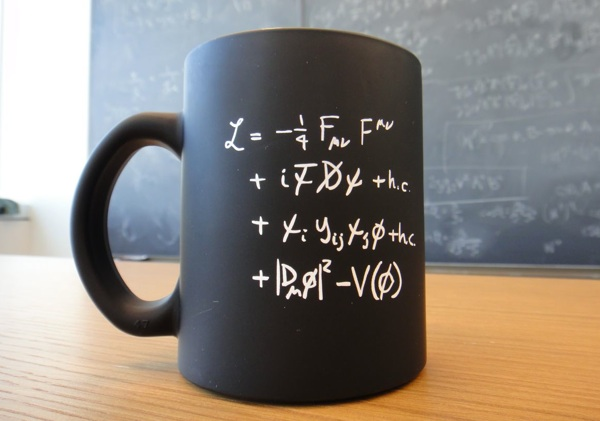
\includegraphics[width=\textwidth]{slides/figures/cernmug.jpeg}
        \column{0.5\textwidth}
        \begin{itemize}
            \item The Standard Model (SM) represents the our current best understanding of the matter and force.
            \item Matters are modeled as fermions: 
            \begin{itemize}
            \smaller
                \item \textcolor{red}{leptons (\Pe\PGne), (\PGm\PGnGm), (\PGt\PGnGt)};
                \item quarks (\PQu\PQd), (\PQc\PQs), (\PQt\PQb).
            \end{itemize}
            \item Forces are modeled as gauge bosons:
            \begin{itemize}
            \smaller
                \item eletroweak force \PGg, \PZ, \textcolor{red}{\PW};
                \item strong force \Pg.
            \end{itemize}
            \item Masses of fermions and gauge bosons are generated by one Higgs boson.
            % \item Successful in explaining and predicting most experimental observations so far.
        \end{itemize}
    \end{columns}
    
    \vspace{0.05\textheight}
    \begin{itemize}
        \item The interaction between the leptons and \PW boson is encapsulated in the term $i\bar{\psi}\slashed{D}\psi$:
        \begin{equation*} \tiny
            i\bar{\psi}\slashed{D}\psi = 
            \bar{\chi}_L \gamma^\mu \big( i \partial_\mu  - \textcolor{red}{g} \frac{\tau_a}{2} W^a_\mu  -g'\frac{Y}{2} B_\mu \big) \chi_L 
            + \bar{\psi}_R \gamma^\mu \big( i \partial_\mu -g'\frac{Y}{2} B_\mu \big) \psi_R 
            - g_s (\bar{q}\gamma^\mu  T_{a} q) G_\mu^a .
        \end{equation*}
    \end{itemize}
\end{frame}



% -------------
% new frame
% -------------
\begin{frame}{}
\smaller 
    \begin{block}{lepton flavor universality}
    \begin{center}
    \resizebox{0.6\textwidth}{!}{    \feynmandiagram [inline=(d.base), small, horizontal=d to b] {
        a[particle=\PGne] -- [fermion] b [dot] -- [fermion] c[particle=\Pe], 
        b -- [boson, edge label=\PW] d,}; 
    = \qquad
    \feynmandiagram [inline=(d.base), small, horizontal=d to b] {
        a[particle=\PGnGm] -- [fermion] b [dot] -- [fermion] c[particle=\PGm],
        b -- [boson, edge label=\PW] d, }; 
    = \qquad
    \feynmandiagram [inline=(d.base), small, horizontal=d to b] {
        a[particle=\PGnGt] -- [fermion] b [dot] -- [fermion] c[particle=\PGt],
        b -- [boson, edge label=\PW] d,};}
    \end{center}        
    \end{block}

    
    \vspace{0.02\textheight}
    \begin{itemize} 
        \item One of the fundamental assumptions in the SM is that the coupling strength $g$ is the same for all three generations of leptons, $g_\Pe = g_\PGm = g_\PGt \equiv g $, known as Lepton Flavor Universality (LFU) in the weak interaction.
        \item Tests of the SM LFU can be performed by studies of the \alert{leptonic decays of \PW bosons}. The only subtle difference should be from the decay phase space due to different fermion masses. 
        \item In high-energy regime, tests are performed at colliders. (most relevant)
        \begin{itemize} 
        \smaller 
            \item SPS and Tevatron using $\Pp\bar{\Pp}\to \PW$;
            \item LEP using $\Pe\bar{\Pe}\to \PW \PW$;
            \item LHC using $\Pp\Pp \to \PW$ and \textcolor{red}{ $\Pp\Pp \to \ttbar \to \PQb\PW \PAQb\PW$}.
        \end{itemize}
        \item In low-energy regime, some of the most stringent LFU tests come from the charged weak decays of mesons (e.g. \PK, $\pi$, \PD, \PB) and leptonic decays of taus~\cite{Amhis:2019ckw}. While most experiments show high precision agreement with LFU, tensions have been recently observed in the semileptonic decays of \PB mesons by Belle~\cite{Huschle:2015rga, Sato:2016svk, Hirose:2016wfn}, BaBar ~\cite{Lees:2012xj, Lees:2013uzd} and LHCb~\cite{Aaij:2015yra,Aaij:2017uff, Aaij:2017deq}.
    \end{itemize}
\end{frame}



% -------------
% new frame
% -------------
\begin{frame}{}
\smaller
    \begin{center}
    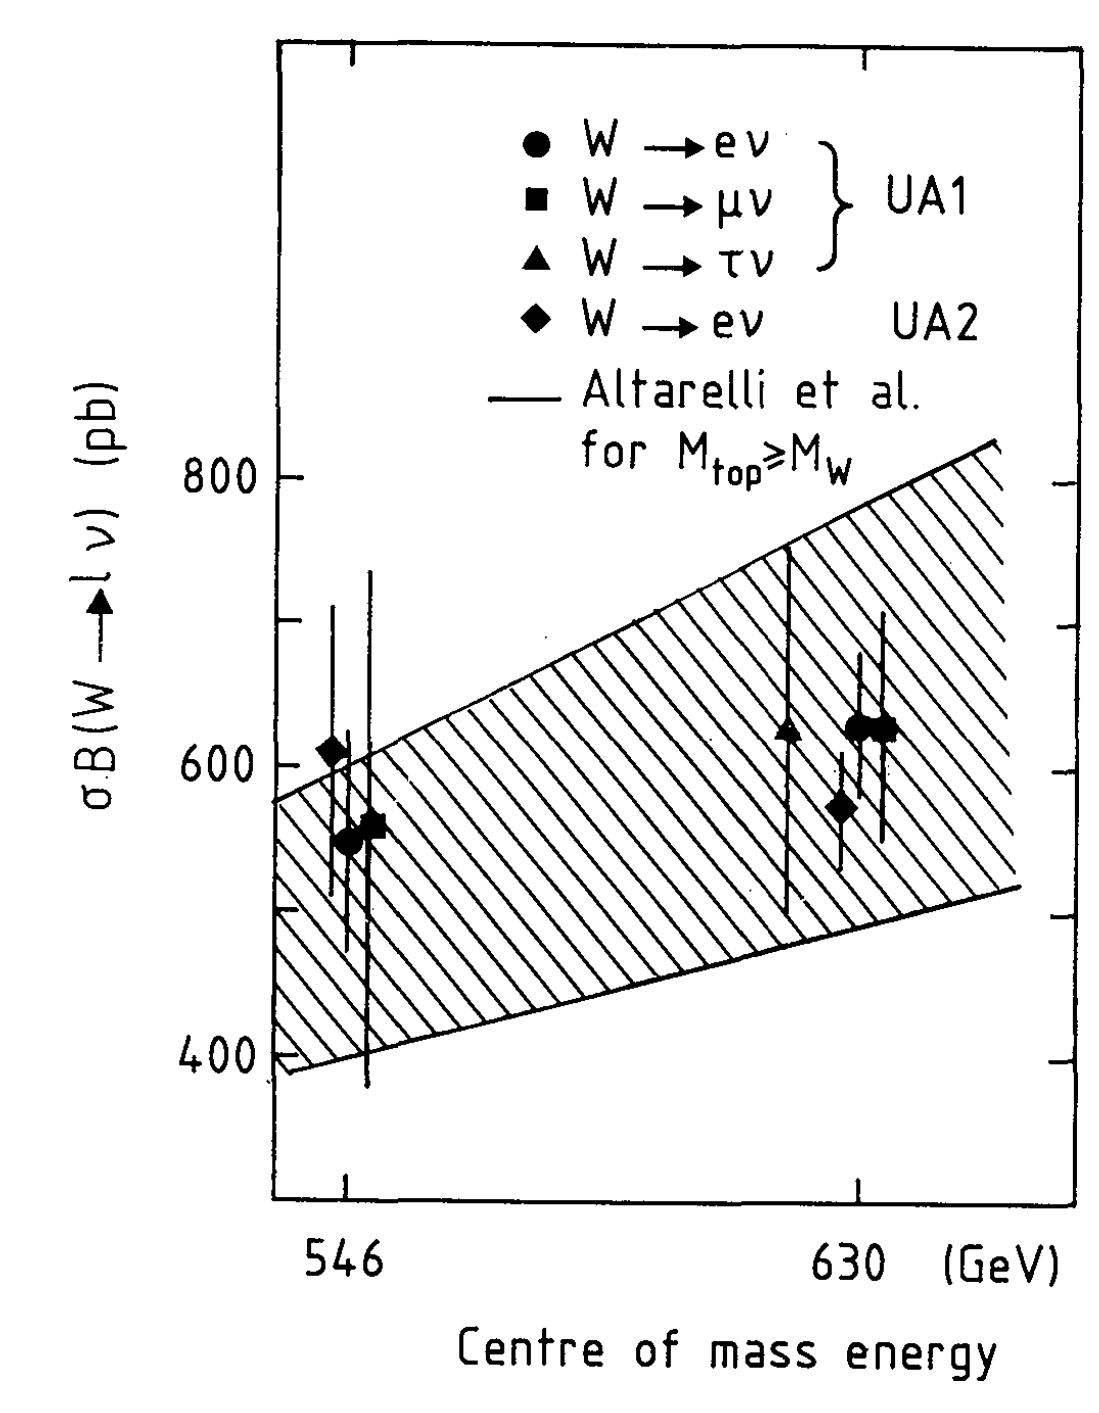
\includegraphics[height=0.4\textheight]{chapters/Introduction/sectionRelatedWorks/figures/sps.png} \qquad
    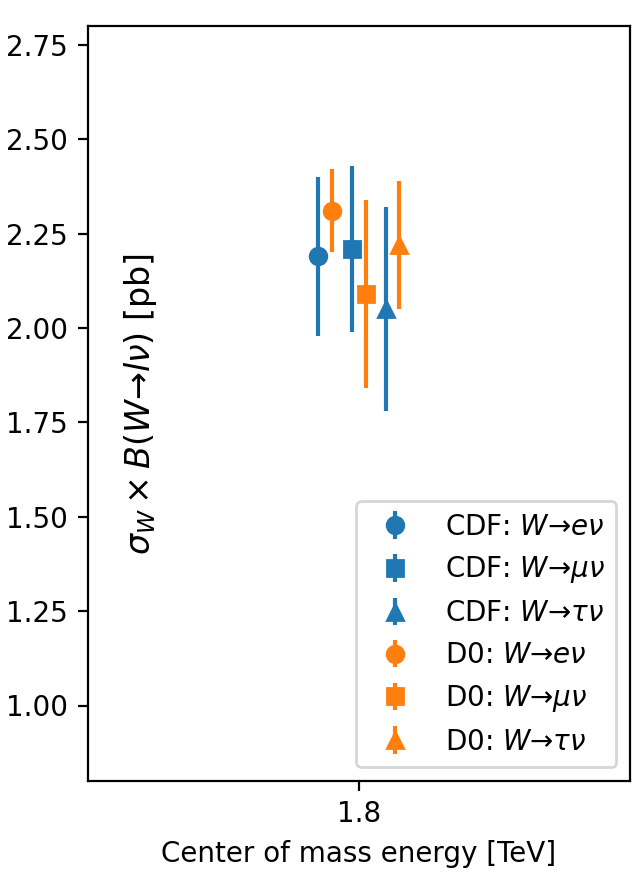
\includegraphics[height=0.4\textheight]{chapters/Introduction/sectionRelatedWorks/figures/tevatron.png}
    \end{center}
    
    \begin{block}{SPS and Tevatron}
        \begin{columns}
            % add column
            \column{0.6\textwidth}
            \begin{itemize}
                \item Measure $\sigma_{\Pp\bar{\Pp}\to \PW} \times \BWemt$.
                \item UA1~\cite{Albajar:1988ka}, UA2~\cite{appel1986measurement, Alitti:1991eh, Alitti:1992hv}, CDF~\cite{Abe:1990sd, Abe:1992ys, Abe:1991fb}, D0~\cite{Abbott:1999tt, Abazov:2003sv, Abachi:1995xc, Abbott:1999pk}.
                \item Taus were reconstructed in the hadronic decay modes.
                \item Combined average $g^\PW_\PGt / g^\PW_\Pe = 0.988\pm 0.025$ (by \DZERO~\cite{Abbott:1999pk}) was consistent with SM.  
            \end{itemize}
            
            % add column
            \column{0.35\textwidth}
            \centering
            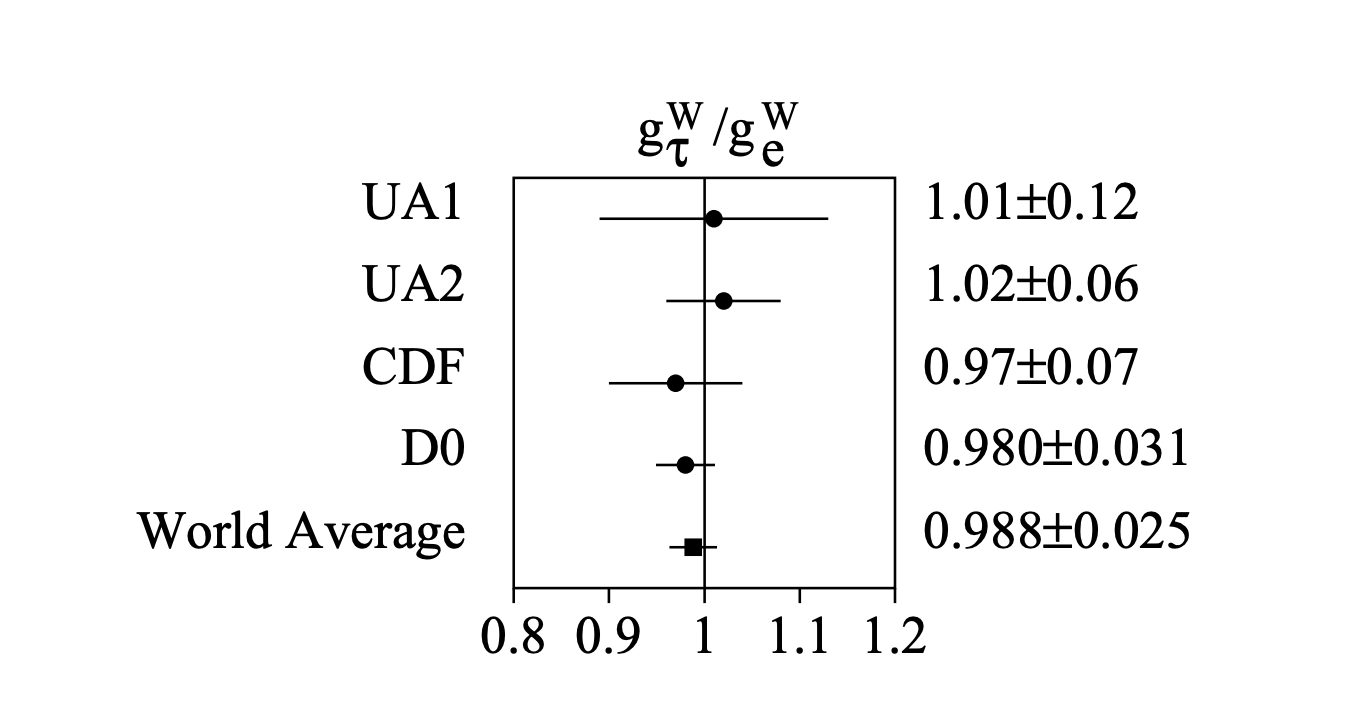
\includegraphics[width=\textwidth]{chapters/Introduction/sectionRelatedWorks/figures/spsTevatron.png}
        \end{columns}
    \end{block}
\end{frame}



% -------------
% new frame
% -------------
\begin{frame}{}
\smaller
    \begin{block}{LEP-II}
        \begin{columns}
            % add column
            \column{0.6\textwidth}
            \begin{itemize}
                \item Measure $\BWemt$ simultaneously.
                \item OPAL~\cite{Abbiendi:2007rs}, DELPHI~\cite{Abdallah:2003zm}, L3~\cite{Achard:2004zw}, ALEPH~\cite{Heister:2004wr}.
                % \item Taus were reconstructed in the hadronic decay modes.
                \item The \alert{most precise and the only} simultaneous \BWemt measurement before our analysis.
                \item The LEP combined result~\cite{Schael:2013ita} showed agreement between electron and muon channel, but tau channel was \alert{$2.6 \; \sigma$} above the average $$ \tiny 2\BWt/ \BWem = 1.066 \pm 0.025 $$ comparing with the SM prediction 0.999~\cite{Denner:1991kt,Rtau,dEnterria:2016rbf}.
            \end{itemize}
            
            % add column
            \column{0.35\textwidth}
            \centering
            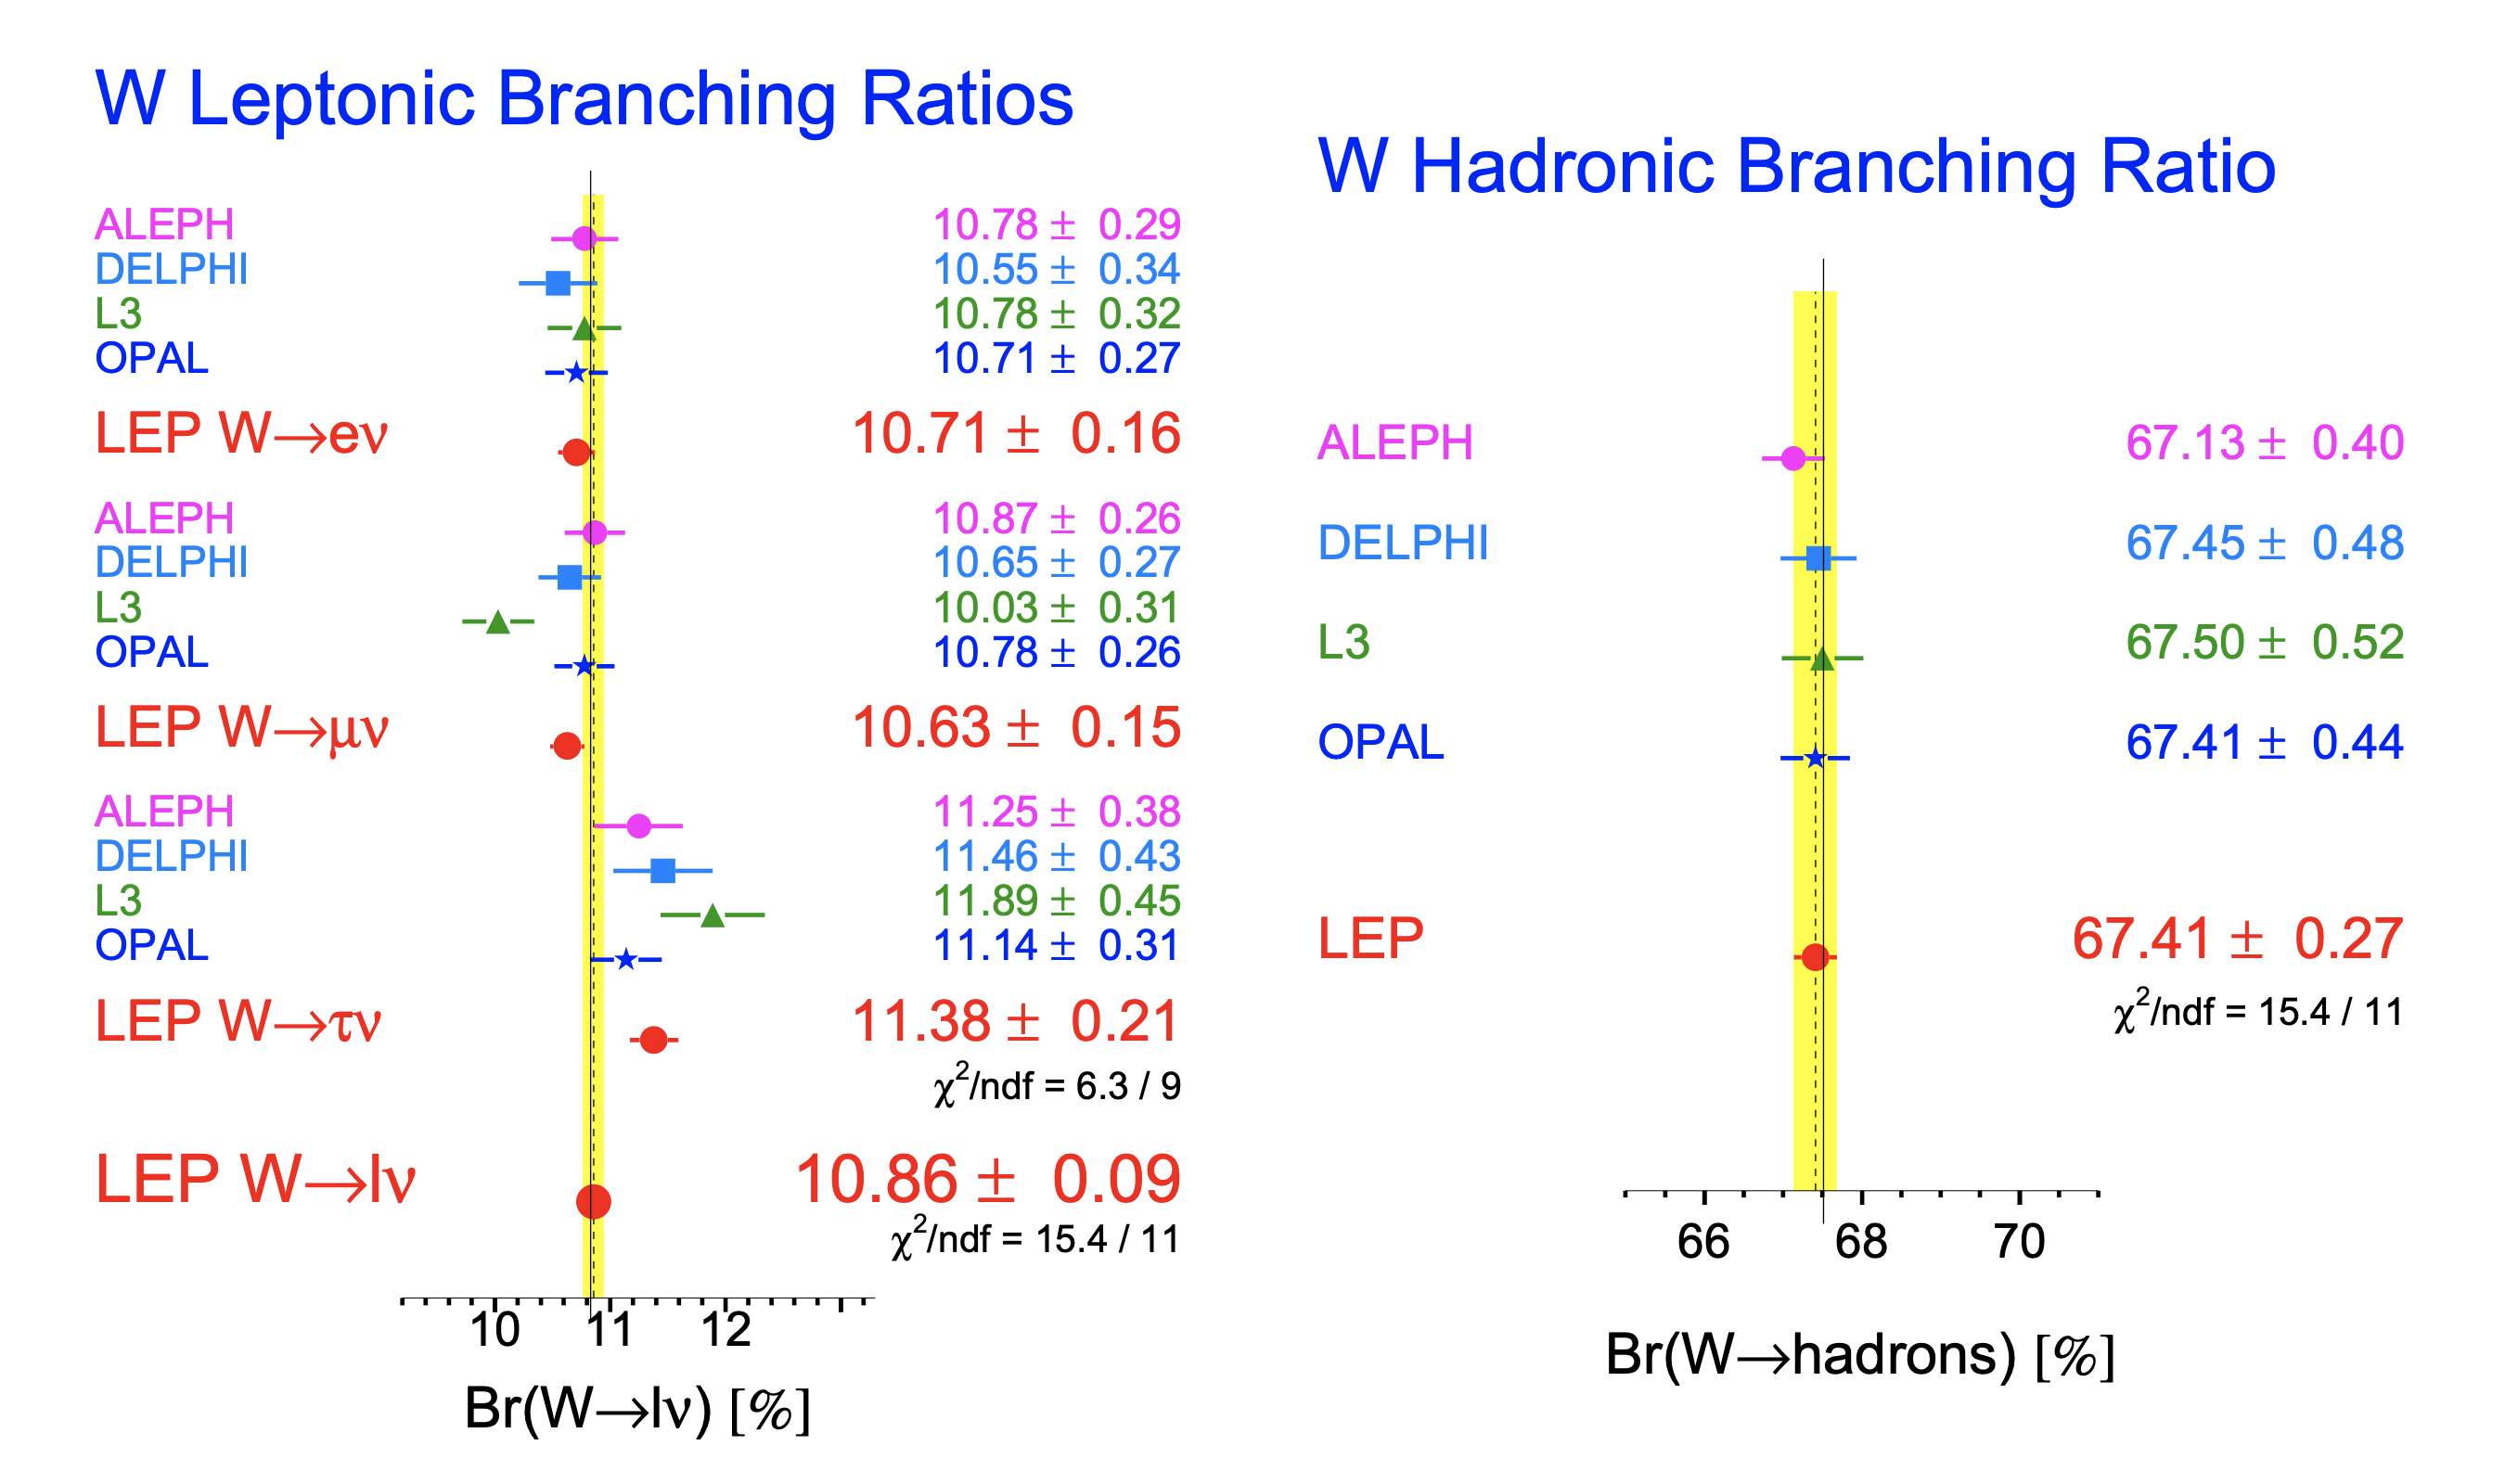
\includegraphics[width=\textwidth, trim=0 0 25cm 0, clip]{chapters/Introduction/sectionRelatedWorks/figures/lep.png}
        \end{columns}
    \end{block}
\end{frame}





% -------------
% new frame
% -------------
\begin{frame}{}
\smaller
    \begin{block}{LHC run-1}
        At $\sqrt{s}=$ 7\TeV and 8\TeV, the LFU between $\PW \to \Pe \PGn$ and $\PW \to \PGm \PGn$ was tested by ATLAS~\cite{Aaboud:2016btc} and LHCb~\cite{Aaij:2015zlq, Aaij:2016qqz}.
        \begin{itemize}
            \item Measure \wjets cross-section in electron and muon channels
            \item The ratio led to $R^{\PW}_{\PGm/\Pe} = 1.003\pm 0.010 ~\mathrm(ATLAS)$  and  $0.980\pm 0.018 ~\mathrm(LHCb)$.
        \end{itemize}
    \end{block}
                
   \begin{block}{LHC run-2}
        \begin{columns}[c]
            % add column
            \column{0.6\textwidth}           
            At $\sqrt{s}=$ 13\TeV, ATLAS~\cite{Aad:2020ayz} has most recently published a test between muon and tau.
            \begin{itemize}
            \smaller
                \item Measure $R^{\PW}_{\PGt/\PGm}$ with the best precision.
                \item Use $\Pp\Pp\to\ttbar\to\PQb\PW\PAQb\PW$ events selected with \cmm, \cem plus two \PQb tagged jets final states.
                \item Tau leptons are probed via their muonic final state $\PGt\to\PGm\PAGnGm\PGnGt$, softer and more displaced than prompt ones.
                \item Fit the muon transverse displacement in three \pt bins. The result indicates LFU. $ \tiny R^{\PW}_{\PGt/\PGm} = 0.992 \pm 0.013 $.
                \item Ease LEP's tension, but individual \BWemt are not measured.
            \end{itemize}
            
            % add column
            \column{0.35\textwidth}
            \centering
            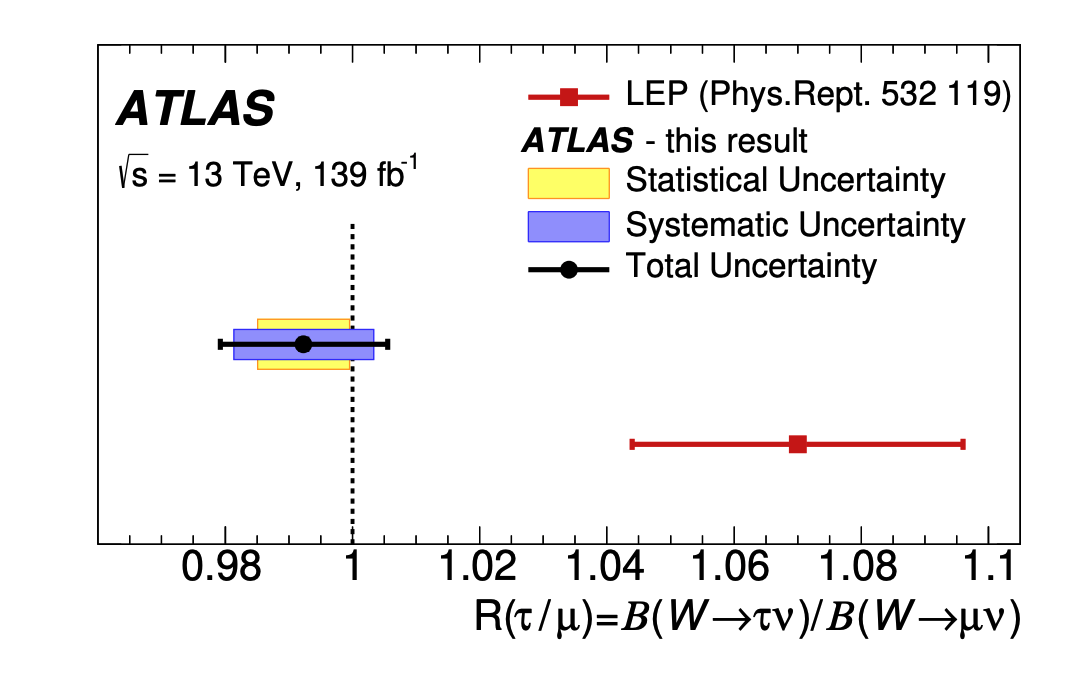
\includegraphics[width=\textwidth]{chapters/Introduction/sectionRelatedWorks/figures/atlas.png}
        \end{columns}
    \end{block}
\end{frame}






% -------------
% new frame
% -------------
\begin{frame}{This analysis}
\smaller
    \begin{columns}
        % add column
        \column{0.55\textwidth}
        \begin{block}{}
            \centering
            \small{\ttbar} process
            \resizebox{0.98\textwidth}{!}{    \feynmandiagram[small,horizontal=a to b]{
        i1 [particle=\PQq] -- [fermion] a -- [fermion] i2 [particle=\PQq],
        a -- [gluon, edge label=\Pg] b,
        f1 [particle=\PQt] -- [fermion] b -- [fermion] f2 [particle=\PQt],
        % top decay
        f1b[particle=\PQb] -- [fermion] f1 -- [photon] f1W [particle=\PW, red],
        f2b[particle=\PQb] -- [anti fermion] f2 -- [photon] f2W [particle=\PW, red],
        f1 -- [opacity=0.0] f2,
        f1W -- [opacity=0.0] f2W,
        f1b -- [opacity=0.0] f1W,
        f2b -- [opacity=0.0] f2W,
    }; \qquad
    \feynmandiagram[small,horizontal=a to b]{
        i1 [particle=\Pg] -- [gluon] a -- [gluon] i2 [particle=\Pg],
        a -- [gluon, edge label=\Pg] b,
        f1 [particle=\PQt] -- [fermion] b -- [fermion] f2 [particle=\PQt],
        % top decay
        f1b[particle=\PQb] -- [fermion] f1 -- [photon] f1W [particle=\PW, red],
        f2b[particle=\PQb] -- [anti fermion] f2 -- [photon] f2W [particle=\PW, red],
        f1 -- [opacity=0.0] f2,
        f1W -- [opacity=0.0] f2W,
        f1b -- [opacity=0.0] f1W,
        f2b -- [opacity=0.0] f2W,
    }; \qquad
    \feynmandiagram[small, vertical=a to b, horizontal=a to f1]{
        i1 [particle=\Pg] -- [gluon] a -- [anti fermion] f1 [particle=\PQt],
        a -- [fermion, edge label=\PQt] b,
        i2 [particle=\Pg] -- [gluon] b -- [fermion] f2 [particle=\PQt],
        % top decay
        f1b[particle=\PQb] -- [fermion] f1 -- [photon] f1W [particle=\PW, red],
        f2b[particle=\PQb] -- [anti fermion] f2 -- [photon] f2W [particle=\PW, red],
        f1 -- [opacity=0.0] f2,
        f1W -- [opacity=0.0] f2W,
        f1b -- [opacity=0.0] f1W,
        f2b -- [opacity=0.0] f2W,
        % i1 -- [opacity=0.0] i2,
        % f1 -- [opacity=0.0] f2,
    };}
        \end{block}
        % add column
        \column{0.4\textwidth}
        \begin{block}{}
            \centering
            \small{\tW} process
            \resizebox{0.98\textwidth}{!}{    \feynmandiagram[scale=0.7][horizontal=a to b]{
        i1 [particle=\PQb] -- [fermion] a -- [gluon] i2 [particle=\Pg],
        a -- [fermion, edge label=\PQb] b,
        f1 [particle=\PW , red] -- [photon] b -- [fermion] f2 [particle=\PQt],
        f2b[particle=\PQb] -- [anti fermion] f2 -- [photon] f2W [particle=\PW, red],
        f1 -- [opacity=0.0] f2W,
    }; \qquad
    \feynmandiagram[scale=0.7][vertical=a to b]{
        i1 [particle=\PQb] -- [fermion] a -- [photon] f1 [particle=\PW, red],
        a -- [fermion, edge label=\PQb] b,
        i2 [particle=\Pg] -- [gluon] b -- [fermion] f2 [particle=\PQt],
        f2b[particle=\PQb] -- [anti fermion] f2 -- [photon] f2W [particle=\PW, red],
        i1 -- [opacity=0.0] i2,
        f1 -- [opacity=0.0] f2W -- [opacity=0.0] f2b,
    };}
        \end{block}
    \end{columns}
    
    % \vspace{0.1\textheight}
    \begin{itemize}
        \item Our analysis presents a simultaneous measurement of three individual \BWemt with the CMS.
        \begin{itemize} 
        \smaller
            \item use run 2016 dataset from the LHC $\sqrt{s}=13\TeV$ proton-proton collisions;
            \item treat \ttbar and \tW processes as the primary signals (WW also considered);
            \item single electron trigger and single muon trigger.
        \end{itemize} 
        
        \item Motivations:
        \begin{itemize} 
        \smaller
            \item the \BWemt measurements have not been improved for more than a decade since LEP;
            \item LEP's $R_{\PGt/(\Pe,\PGm)}$ shows a $2.6\,\sigma$ deviation from the SM prediction.
        \end{itemize}
        \item Opportunities:
        \begin{itemize} 
        \smaller
            \item LHC 13\TeV collisions produce an unprecedentedly large number of \ttbar events giving $\PW\PW$ pairs;
            \item the \PQb tagging allows to select \ttbar events with a high purity;
            \item the improved \PGth identification enables to efficiently select \PW tauonic decays.
        \end{itemize}
    \end{itemize}
\end{frame}
    
    
    
\begin{frame}{This analysis}
\smaller
    \begin{block}{two approaches}
        
    \begin{itemize}
        \item Shape analysis:
        \begin{itemize}
        \smaller
            \item template fit the \pt distribution of the sensitive leptons in all different channels simultaneously;
            \item to improve the precision from LEP.
        \end{itemize}
    
        \item Counting analysis:
        \begin{itemize}
        \smaller
            \item construct ratios of yields for channels with the same trigger and solve three leptonic branching fractions from a set of quadratic equations;
            \item to cross-check with the shape analysis.
        \end{itemize}
    \end{itemize}
    \end{block}
    
    
    \begin{itemize}
        \item Primarily measure three individual leptonic branching fraction $$\BWe \quad \BWm \quad \BWt$$
        \item Additional derived quantities
        \begin{itemize}
        \smaller
            \item assuming partial LFU between \Pe and \PGm, measures the ratio $R^{\PW}_{\PGt/(\Pe,\PGm)}$;
            \item assuming LFU, the average leptonic and inclusive hadronic branching fraction;
            \item assuming LFU, three the SM quantities, $\alpS$, \sumCKM, \absVcs, are derived from \BWh.
        \end{itemize}
    \end{itemize}
\end{frame}
      
        %     \textbf{}      &  \\ 
        % \hline
        % \textbf{Counting analysis}   & 
% \begin{frame}{Introduction}
%     \begin{center}
%     \begin{itemize} \smaller
%         \item A
%         \item B
%     \end{itemize}
%     \end{center}
    
%     \begin{center}
%     \begin{columns}
%         % add column
%         \column{0.4\textwidth}
%         add column
        
%         % add column
%         \column{0.6\textwidth}
%         add column
%     \end{columns}
%     \end{center}
% \end{frame}
    

            

        

